%=============================================%
%=                                           =%
%=           ..:: STAR BATTLE ::..           =%
%=                                           =%
%=============================================%
%=                                           =%
%=             ..:: Authors ::..             =%
%=                                           =%
%=     Henrique Ferrolho && Joao Pereira     =%
%=                FEUP - 2014                =%
%=                                           =%
%=============================================%

\documentclass[runningheads,a4paper]{llncs}

\usepackage[portuguese]{babel}
\usepackage[utf8]{inputenc}
\usepackage{amssymb}
\setcounter{tocdepth}{3}
\usepackage{graphicx}

\usepackage{url}
\urldef{\mailsa}\path|{alfred.hofmann, ursula.barth, ingrid.haas, frank.holzwarth,|
\urldef{\mailsb}\path|anna.kramer, leonie.kunz, christine.reiss, nicole.sator,|
\urldef{\mailsc}\path|erika.siebert-cole, peter.strasser, lncs}@springer.com|    
\newcommand{\keywords}[1]{\par\addvspace\baselineskip
\noindent\keywordname\enspace\ignorespaces#1}

\begin{document}

\mainmatter  % start of an individual contribution

\title{Star Battle}
\subtitle{Resolução de Problema de Decisão usando\\
Programação em Lógica com Restrições}
\titlerunning{Star Battle}

\author{Henrique Ferrolho\and João Pereira}
\authorrunning{Henrique Ferrolho\and João Pereira}

\institute{Faculdade de Engenharia da Universidade do Porto\\
Rua Roberto Frias, sn, 4200-465 Porto, Portugal\\}

\toctitle{Star Battle}
\maketitle


\begin{abstract}
Este artigo complementa o segundo projecto da Unidade Curricular de Programação em Lógica, do Mestrado Integrado em Engenharia Informática e de Computação. O projecto consiste num programa, escrito em Prolog, capaz de resolver qualquer tabuleiro do jogo Star Battle, que é um problema de decisão.
\keywords{star battle, sicstus, prolog, feup}
\end{abstract}


\section{Introdução}

asdasdad

asdads

\section{Descrição do Problema}


\section{Abordagem}

\subsection{Variáveis de Decisão}

\subsection{Restrições}

\subsection{Função de Avaliação}


\section{Visualização da Solução}

\begin{figure}
\centering
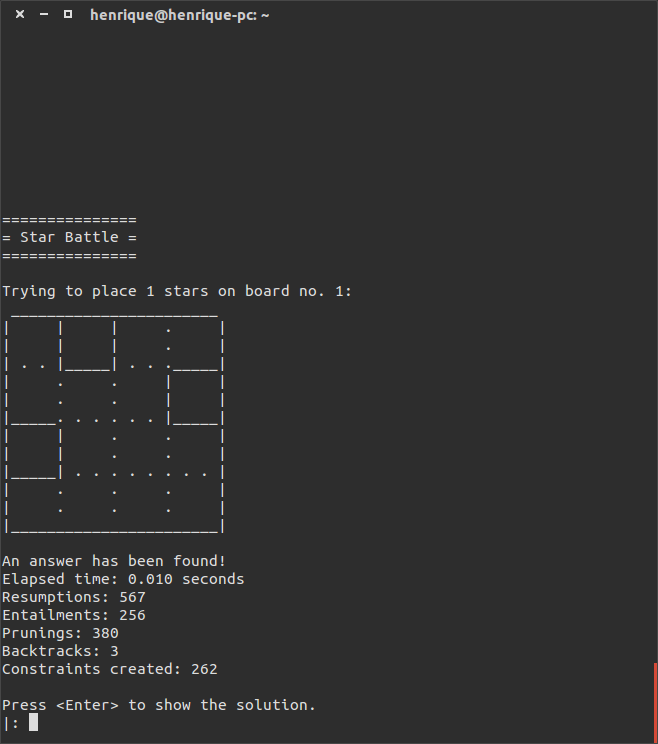
\includegraphics[height=6.2cm]{res/testBoard4x4_1}
\caption{caption.}
\label{fig:example}
\end{figure}

\begin{figure}
\centering
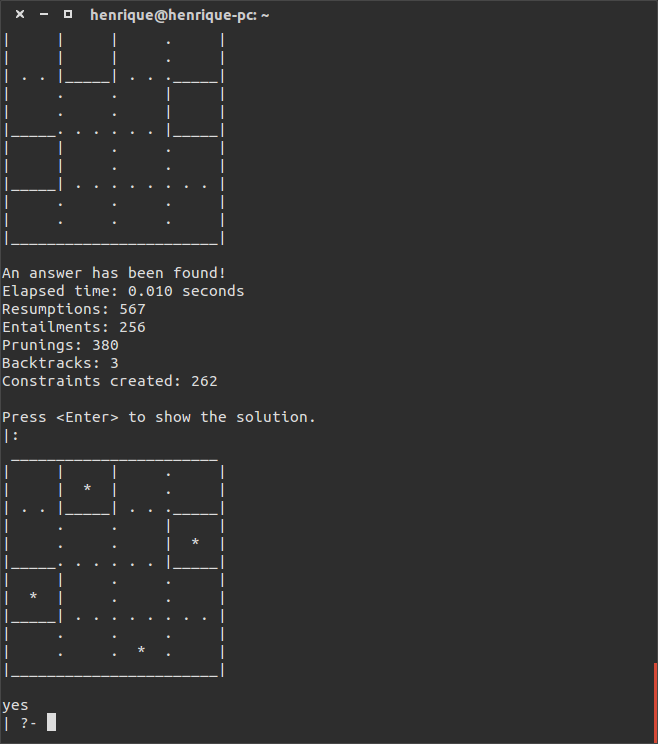
\includegraphics[height=6.2cm]{res/testBoard4x4_1-solution}
\caption{caption.}
\label{fig:example}
\end{figure}


\section{Resultados}

\section{Conclusões}

Escrever conclusões aqui


\begin{thebibliography}{4}

\bibitem{url} Star Battle rules,\\
\url{http://logicmastersindia.com/lmitests/dl.asp?attachmentid=430}

\bibitem{url} SICStus Prolog, \url{https://sicstus.sics.se/}

\bibitem{url} SWI-Prolog, \url{http://www.swi-prolog.org/}

\end{thebibliography}


\section*{Anexo}

\subsection*{Código fonte}

\newenvironment{changemargin}[2]{%
\begin{list}{}{%
\setlength{\topsep}{0pt}%
\setlength{\leftmargin}{#1}%
\setlength{\rightmargin}{#2}%
\setlength{\listparindent}{\parindent}%
\setlength{\itemindent}{\parindent}%
\setlength{\parsep}{\parskip}%
}%
\item[]}{
\end{list}}

\medskip

\noindent
{\it starBattle.pl}
\begin{changemargin}{-3cm}{-4cm}
\begin{verbatim}

%=============================================%
%=                                           =%
%=           ..:: STAR BATTLE ::..           =%
%=                                           =%
%=        Type 'starBattle.' to start        =%
%=                                           =%
%=============================================%
%=                                           =%
%=             ..:: Authors ::..             =%
%=                                           =%
%=     Henrique Ferrolho && Joao Pereira     =%
%=                FEUP - 2014                =%
%=                                           =%
%=============================================%

%===============%
%= @@ includes =%
%===============%
:- use_module(library(clpfd)).
:- include('containers.pl').
:- include('printer.pl').
:- include('solver.pl').
:- include('starBattleTestBoards.pl').
:- include('utilities.pl').

%====================%
%= @@ game launcher =%
%====================%
starBattle:-
    clearConsole,
    write('To run the program type:'), nl,
    nl,
    write('\tstarBattle(NumBoard, NumStars).'),nl,
    nl,
    write('- NumBoard'), nl,
    write('number of the board you wish to test.'), nl,
    nl,
    write('- NumStars'), nl,
    write('number of stars you wish to place on each row, column and region.'), nl,
    nl.

starBattle(BoardNumber, NumStars):-
    clearConsole,
    write('==============='), nl,
    write('= Star Battle ='), nl,
    write('==============='), nl,
    nl,
    format('Trying to place ~d stars on board no. ~d:', [NumStars, BoardNumber]), nl,

    getBoard(BoardNumber, Board),
    printBoard(Board), !,

    solveBoard(Board, NumStars, Result), !,
    pressEnterToContinue,

    %getBoardSize(Board, BoardSize),
    %printResult(Result, BoardSize, NumStars),
    printResultBoard(Board, Result, NumStars), !.
    
    
\end{verbatim}
\end{changemargin}

\noindent
{\it solver.pl}
\begin{changemargin}{-3cm}{-4cm}
\begin{verbatim}

solveBoard(Board, S, Result):-
    getBoardSize(Board, N),

    % a board NxN can not have more than N/2 stars
    S #=< (N - 1) // 2 + 1,

    ResultLength #= N * S,

    length(Result, ResultLength),
    length(ResultRegions, ResultLength),

    domain(Result, 1, N),
    domain(ResultRegions, 1, N),

    % 1st restriction
    validateNumOfOccurrencesForEachElem(Result, S, N),

    % 2nd restriction
    fetchResultRegions(Board, Result, N, S, ResultRegions),
    validateNumOfOccurrencesForEachElem(ResultRegions, S, N),

    % 3rd restriction
    noAdjacentStars(Result, S, N),

    statistics(walltime, _),
    labeling([bisect], Result),
    statistics(walltime, [_, ElapsedTime | _]),
    format('An answer has been found!~nElapsed time: ~3d seconds', ElapsedTime), nl,
    fd_statistics,
    nl.


%-%-%-%-%-%-%-%-%-%-%-%-%-%-%-%-%-%-%-%-%-%-%-%-%-%-%-%-%-%-%-%-%-%-%

getBoardSize([Head|_], N):-
    length(Head, N).


%-%-%-%-%-%-%-%-%-%-%-%-%-%-%-%-%-%-%-%-%-%-%-%-%-%-%-%-%-%-%-%-%-%-%

validateNumOfOccurrencesForEachElem(Elements, NumOfOccurrences, N):-
    validateNumOfOccurrencesForEachElem(Elements, NumOfOccurrences, N, 1).

validateNumOfOccurrencesForEachElem(Result, S, N, N):-
    exactly(N, Result, S).
validateNumOfOccurrencesForEachElem(Result, S, N, I):-
    exactly(I, Result, S),
    I1 #= I + 1,
    validateNumOfOccurrencesForEachElem(Result, S, N, I1).


%-%-%-%-%-%-%-%-%-%-%-%-%-%-%-%-%-%-%-%-%-%-%-%-%-%-%-%-%-%-%-%-%-%-%

fetchResultRegions(Board, Result, ResRows, ResCols, ResultRegions):-
    fetchResultRegions(Board, Result, ResRows, ResCols, [], 1, ResultRegions).

fetchResultRegions(_, _, ResRows, ResCols, ResultRegions, Pos, ResultRegions):-
    Pos #= ResRows * ResCols + 1.
fetchResultRegions(Board, Result, ResRows, ResCols, ResultRegionsSoFar, Pos, ResultRegions):-
    % calculating row and col of result to access
    Row #= (Pos - 1) // ResCols + 1,
    Col #= ((Pos - 1) mod ResCols) + 1,

    % get the value of result[Row][Col], which is the column where a star is placed
    getMatrixOfListElemAt(Result, ResRows, ResCols, Row, Col, StarCol),

    % get line Row of the board
    getListElemAt(Board, Row, Line),

    % get the region of that position - board[Row][StarCol]
    element(StarCol, Line, Region),

    % push value to ResultRegionsSoFar
    listPushBack(ResultRegionsSoFar, Region, NewResultRegionsSoFar),

    % fetch next element
    Pos1 #= Pos + 1,
    fetchResultRegions(Board, Result, ResRows, ResCols, NewResultRegionsSoFar, Pos1, ResultRegions).


%-%-%-%-%-%-%-%-%-%-%-%-%-%-%-%-%-%-%-%-%-%-%-%-%-%-%-%-%-%-%-%-%-%-%

noAdjacentStars(Result, S, N):-
    noAdjacentStars(Result, S, N, 1).

noAdjacentStars(Result, S, N, 1):-
    noAdjacentStarsOnRow(Result, S, 1),
    noAdjacentStars(Result, S, N, 2).
noAdjacentStars(_, _, N, Row):-
    Row #= N + 1.
noAdjacentStars(Result, S, N, Row):-
    Row #> 1,
    noAdjacentStarsOnRow(Result, S, Row),
    noAdjacentStarsWithPreviousRow(Result, S, Row),
    Row1 #= Row + 1,
    noAdjacentStars(Result, S, N, Row1).


%-%-%-%-%-%-%-%-%-%-%-%-%-%-%-%-%-%-%-%-%-%-%-%-%-%-%-%-%-%-%-%-%-%-%

noAdjacentStarsOnRow(Result, S, Row):-
    StartPos #= (Row - 1) * S + 1,
    EndPos #= StartPos + S,
    validateStarsFromStartToEnd(Result, StartPos, EndPos).

validateStarsFromStartToEnd(Result, Start, End):-
    Next #= Start + 1,
    validateStarsFromStartToEnd(Result, Start, Next, End).

validateStarsFromStartToEnd(_, Start, _, End):-
    Start #= End - 1.
validateStarsFromStartToEnd(Result, Start, End, End):-
    Start1 #= Start + 1,
    Next #= Start1 + 1,
    validateStarsFromStartToEnd(Result, Start1, Next, End).
validateStarsFromStartToEnd(Result, Start, Next, End):-
    validateHorizontalDistanceBetweenStars(Result, Start, Next),
    Next1 #= Next + 1,
    validateStarsFromStartToEnd(Result, Start, Next1, End).


%-%-%-%-%-%-%-%-%-%-%-%-%-%-%-%-%-%-%-%-%-%-%-%-%-%-%-%-%-%-%-%-%-%-%

noAdjacentStarsWithPreviousRow(Result, S, Row):-
    StartPos #= (Row - 1) * S + 1,
    EndPos #= StartPos + S,
    noAdjacentStarsWithPreviousRow(Result, S, Row, StartPos, EndPos).

noAdjacentStarsWithPreviousRow(_, _, _, EndPos, EndPos).
noAdjacentStarsWithPreviousRow(Result, S, Row, CurrentPos, EndPos):-
    % for each star of the row being validated,
    % validate horizontal distance to each star of the previous row
    PrevRow #= Row - 1,
    starIsNotAdjacentWithAnyOfThePreviousRow(Result, S, CurrentPos, PrevRow),
    % procceed to next row
    CurrentPos1 #= CurrentPos + 1,
    noAdjacentStarsWithPreviousRow(Result, S, Row, CurrentPos1, EndPos).

starIsNotAdjacentWithAnyOfThePreviousRow(Result, S, PivotStar, PrevRow):-
    FirstStarPos #= (PrevRow - 1) * S + 1,
    LastStarPos #= FirstStarPos + S,
    starIsNotAdjacentToAnyOtherStarFromFirstToLastPos(Result, PivotStar, FirstStarPos, LastStarPos).

starIsNotAdjacentToAnyOtherStarFromFirstToLastPos(_, _, LastStarPos, LastStarPos).
starIsNotAdjacentToAnyOtherStarFromFirstToLastPos(Result, PivotStar, CurrentStarPos, LastStarPos):-
    validateHorizontalDistanceBetweenStars(Result, PivotStar, CurrentStarPos),
    NextStarPos #= CurrentStarPos + 1,
    starIsNotAdjacentToAnyOtherStarFromFirstToLastPos(Result, PivotStar, NextStarPos, LastStarPos).


%-%-%-%-%-%-%-%-%-%-%-%-%-%-%-%-%-%-%-%-%-%-%-%-%-%-%-%-%-%-%-%-%-%-%

validateHorizontalDistanceBetweenStars(Result, Pos1, Pos2):-
    element(Pos1, Result, Col1),
    element(Pos2, Result, Col2),
    Dist #= abs(Col2 - Col1),
    Dist #> 1.
    
    
\end{verbatim}
\end{changemargin}

\noindent
{\it printer.pl}
\begin{changemargin}{-3cm}{-4cm}
\begin{verbatim}

%===============================%
%= @@ board printing functions =%
%===============================%
printBoard(Board):-
    getBoardSize(Board, N),
    printBoardTopBorder(N),
    printBoard(Board, 1, N),
    nl, !.
printResultBoard(Board, Result, S):-
    getBoardSize(Board, N),
    printBoardTopBorder(N),
    printBoard(Board, 1, N, Result, S),
    nl, !.

printBoardTopBorder(N):-
    N1 is N - 1, createSeparatorN(N1, '______', TopBorder),
    write(' '), printList(TopBorder), write('_____'), nl.

printBoard(Board, N, N):-
    printBoardRow(Board, N, N).
printBoard(Board, I, N):-
    printBoardRow(Board, I, N), !,
    I1 is I + 1,
    printBoard(Board, I1, N).
%-%-%-%-%-%-%
printBoard(Board, N, N, Result, S):-
    printBoardRow(Board, N, N, Result, S).
printBoard(Board, I, N, Result, S):-
    printBoardRow(Board, I, N, Result, S), !,
    I1 is I + 1,
    printBoard(Board, I1, N, Result, S).

%-%-%-%-%-%-%-%-%-%-%-%-%-%-%-%-%-%-%-%-%-%-%-%-%-%-%-%-%-%-%-%-%-%-%

printBoardRow(Board, N, N):-
    write('|'), printBoardRowTop(Board, N, N, 1), nl, !,
    write('|'), printBoardRowMiddle(Board, N, N, 1), nl, !,
    write('|'), printBoardLastRowBottom(Board, N, N, 1), nl, !.
printBoardRow(Board, I, N):-
    write('|'), printBoardRowTop(Board, I, N, 1), nl, !,
    write('|'), printBoardRowMiddle(Board, I, N, 1), nl, !,
    write('|'), printBoardRowBottom(Board, I, N, 1), nl, !.
%-%-%-%-%-%-%
printBoardRow(Board, N, N, Result, S):-
    write('|'), printBoardRowTop(Board, N, N, 1), nl, !,
    write('|'), printBoardRowMiddle(Board, N, N, 1, Result, S), nl, !,
    write('|'), printBoardLastRowBottom(Board, N, N, 1), nl, !.
printBoardRow(Board, I, N, Result, S):-
    write('|'), printBoardRowTop(Board, I, N, 1), nl, !,
    write('|'), printBoardRowMiddle(Board, I, N, 1, Result, S), nl, !,
    write('|'), printBoardRowBottom(Board, I, N, 1), nl, !.

%-%-%-%-%-%-%-%-%-%-%-%-%-%-%-%-%-%-%-%-%-%-%-%-%-%-%-%-%-%-%-%-%-%-%

printBoardRowTop(_, _, N, N):-
    write('     |').
printBoardRowTop(Board, I, N, Col):-
    getListElemAt(Board, I, Row),
    Col1 is Col + 1,
    element(Col, Row, V1),
    element(Col1, Row, V2),
    printCellTop(V1, V2),
    printBoardRowTop(Board, I, N, Col1).

% @@@ swap comment to toggle region display
%printBoardRowMiddle(Board, I, N, N):-
%   getListElemAt(Board, I, Row),
%   element(N, Row, V1),
%   write('  '), write(V1), write('  |').
printBoardRowMiddle(_, _, N, N):-
    write('     |').
printBoardRowMiddle(Board, I, N, Col):-
    getListElemAt(Board, I, Row),
    Col1 is Col + 1,
    element(Col, Row, V1),
    element(Col1, Row, V2),
    printValue(V1, V2),
    printBoardRowMiddle(Board, I, N, Col1).
%-%-%-%-%-%-%
printBoardRowMiddle(_, I, N, N, Result, S):-
    starExistsIn(Result, S, I, N),
    write('  *  |').
printBoardRowMiddle(_, _, N, N, _, _):-
    write('     |').
printBoardRowMiddle(Board, I, N, Col, Result, S):-
    starExistsIn(Result, S, I, Col),

    getListElemAt(Board, I, Row),
    Col1 is Col + 1,
    element(Col, Row, V1),
    element(Col1, Row, V2),
    printStar(V1, V2),
    printBoardRowMiddle(Board, I, N, Col1, Result, S).
printBoardRowMiddle(Board, I, N, Col, Result, S):-
    getListElemAt(Board, I, Row),
    Col1 is Col + 1,
    element(Col, Row, V1),
    element(Col1, Row, V2),
    printValue(V1, V2),
    printBoardRowMiddle(Board, I, N, Col1, Result, S).

printBoardRowBottom(Board, I, N, N):-
    getListElemAt(Board, I, Row),
    I1 is I + 1, getListElemAt(Board, I1, NextRow),

    element(N, Row, V1),
    element(N, NextRow, V3),

    printCellBottom(V1, V3).
printBoardRowBottom(Board, I, N, Col):-
    getListElemAt(Board, I, Row),
    I1 is I + 1, getListElemAt(Board, I1, NextRow),
    NextCol is Col + 1,

    element(Col, Row, V1),
    element(NextCol, Row, V2),
    element(Col, NextRow, V3),

    printCellBottom(V1, V2, V3),
    printBoardRowBottom(Board, I, N, NextCol).

printBoardLastRowBottom(_, _, N, N):-
    write('_____|').
printBoardLastRowBottom(Board, I, N, Col):-
    getListElemAt(Board, I, Row),
    NextCol is Col + 1,

    element(Col, Row, V1),
    element(NextCol, Row, V2),

    printLastRowCellBottom(V1, V2),
    printBoardLastRowBottom(Board, I, N, NextCol).

%-%-%-%-%-%-%-%-%-%-%-%-%-%-%-%-%-%-%-%-%-%-%-%-%-%-%-%-%-%-%-%-%-%-%

printCellTop(V1, V1):-
    write('     .').
printCellTop(_, _):-
    write('     |').

% @@@ swap comment to toggle region display
%printValue(V, V):-
%   write('  '), write(V), write('  .').
printValue(V, V):-
    write('     .').

% @@@ swap comment to toggle region display
%printValue(V, _):-
%   write('  '), write(V), write('  |').
printValue(_, _):-
    write('     |').

printStar(V, V):-
    write('  *  .').
printStar(_, _):-
    write('  *  |').

printCellBottom(V, V, V):-
    write(' . . .').
printCellBottom(V, V, _):-
    write('_____.').
printCellBottom(V, _, V):-
    write(' . . |').
printCellBottom(_, _, _):-
    write('_____|').

printCellBottom(V, V):-
    write(' . . |').
printCellBottom(_, _):-
    write('_____|').

printLastRowCellBottom(V, V):-
    write('______').
printLastRowCellBottom(_, _):-
    write('_____|').


%-%-%-%-%-%-%-%-%-%-%-%-%-%-%-%-%-%-%-%-%-%-%-%-%-%-%-%-%-%-%-%-%-%-%

createSeparatorN(0, _, []).
createSeparatorN(N, SS, [SS | Ls]):-
    N1 is N-1,
    createSeparatorN(N1, SS, Ls).


%-%-%-%-%-%-%-%-%-%-%-%-%-%-%-%-%-%-%-%-%-%-%-%-%-%-%-%-%-%-%-%-%-%-%

starExistsIn(Result, S, Row, StarCol):-
    StartPos is (Row - 1) * S + 1,
    EndPos is StartPos + S,
    starExistsSomewhereBetween(Result, StartPos, EndPos, StarCol).

starExistsSomewhereBetween(Result, CurrentPos, _, StarCol):-
    element(CurrentPos, Result, ScanRes),
    StarCol =:= ScanRes.
starExistsSomewhereBetween(Result, CurrentPos, EndPos, StarCol):-
    NextPos is CurrentPos + 1,
    NextPos < EndPos,
    starExistsSomewhereBetween(Result, NextPos, EndPos, StarCol).


%================================%
%= @@ result printing functions =%
%================================%
printResult(Result, N, S):-
    write('Result:'), nl,
    printResultRow(Result, N, S, 1).


printResultRow(Result, N, S, N):-
    write('\t'), printResultRowValues(Result, N, S, N, 1).

printResultRow(Result, N, S, Row):-
    write('\t'), printResultRowValues(Result, N, S, Row, 1),

    Row1 is Row + 1,
    printResultRow(Result, N, S, Row1).


printResultRowValues(Result, _, S, Row, S):-
    Pos is (Row - 1) * S + S,
    getListElemAt(Result, Pos, Elem),
    write(Elem), nl.

printResultRowValues(Result, N, S, Row, Column):-
    Pos is (Row - 1) * S + Column,
    getListElemAt(Result, Pos, Elem),
    write(Elem), write(', '),

    Column1 is Column + 1,
    printResultRowValues(Result, N, S, Row, Column1).
    
    
\end{verbatim}
\end{changemargin}

\noindent
{\it containers.pl}
\begin{changemargin}{-3cm}{-4cm}
\begin{verbatim}

%=================%
%= @@ containers =%
%=================%
% containers are indexed starting at 1, not 0.

%%% 1. matrix; 2. element row; 3. element column; 4. query element.
getMatrixElemAt([ListAtTheHead|_], 1, ElemCol, Elem):-
    getListElemAt(ListAtTheHead, ElemCol, Elem).
getMatrixElemAt([_|RemainingLists], ElemRow, ElemCol, Elem):-
    ElemRow > 1,
    ElemRow1 is ElemRow - 1,
    getMatrixElemAt(RemainingLists, ElemRow1, ElemCol, Elem).

% treats list as if it was a matrix of NRows x NCols and returns the Elem at ElemRow, ElemCol
getMatrixOfListElemAt(List, NRows, NCols, ElemRow, ElemCol, Elem):-
    ElemRow =< NRows, ElemCol =< NCols,
    Pos is (ElemRow - 1) * NCols + ElemCol,
    element(Pos, List, Elem).

%%% 1. list; 2. element position; 3. query element.
getListElemAt([ElemAtTheHead|_], 1, ElemAtTheHead).
getListElemAt([_|RemainingElems], Pos, Elem):-
    Pos > 1,
    Pos1 is Pos - 1,
    getListElemAt(RemainingElems, Pos1, Elem).

listPushBack([], Elem, [Elem]).
listPushBack([Head|Tail], Elem, [Head|NewTail]):-
    listPushBack(Tail, Elem, NewTail).

printList([]).
printList([Head|Tail]):-
    write(Head), printList(Tail).
    
    
\end{verbatim}
\end{changemargin}

\noindent
{\it utilities.pl}
\begin{changemargin}{-3cm}{-4cm}
\begin{verbatim}

%================%
%= @@ utilities =%
%================%
clearConsole:-
    clearConsole(40), !.
clearConsole(0).
clearConsole(N):-
    nl,
    N1 is N-1,
    clearConsole(N1).

pressEnterToContinue:-
    write('Press <Enter> to show the solution.'), nl,
    waitForEnter, !.
waitForEnter:-
    get_char(_).

exactly(_, [], 0).
exactly(X, [Y|L], N) :-
    X #= Y #<=> B,
    N #= M + B,
    exactly(X, L, M).
    
    
\end{verbatim}
\end{changemargin}

\noindent
{\it starBattleTestBoards.pl}
\begin{changemargin}{-3cm}{-4cm}
\begin{verbatim}

%=======================================%
%= @@ function to retrieve test boards =%
%=======================================%
getBoard(N, Board):-
    (
        N =:= 1 -> testBoard4x4_1(Board);
        N =:= 2 -> testBoard5x5_1(Board);
        N =:= 3 -> testBoard5x5_2(Board);
        N =:= 4 -> testBoard8x8_1(Board);
        N =:= 5 -> testBoard8x8_2(Board);
        N =:= 6 -> testBoard10x10_1(Board);
        N =:= 7 -> testBoard10x10_2(Board);

        nl,
        write('Error: the specified board does not exist.'),
        fail
    ).

%==================%
%= @@ test boards =%
%==================%
% expected answer:2413
testBoard4x4_1([
    [1, 2, 1, 1],
    [1, 1, 1, 3],
    [4, 1, 1, 1],
    [1, 1, 1, 1]]).

% expected answer: 14253
testBoard5x5_1([
    [1, 1, 2, 2, 2],
    [1, 2, 2, 3, 2],
    [1, 2, 2, 2, 2],
    [4, 2, 4, 2, 5],
    [4, 4, 4, 5, 5]]).

testBoard5x5_2([
    [1, 1, 1, 2, 2],
    [1, 3, 3, 3, 4],
    [1, 1, 3, 3, 4],
    [1, 5, 5, 5, 5],
    [1, 1, 1, 5, 5]]).

% expected answer: 2468246813571357
testBoard8x8_1([
    [1, 2, 3, 4, 5, 6, 7, 8],
    [1, 2, 3, 4, 5, 6, 7, 8],
    [1, 2, 3, 4, 5, 6, 7, 8],
    [1, 2, 3, 4, 5, 6, 7, 8],
    [1, 2, 3, 4, 5, 6, 7, 8],
    [1, 2, 3, 4, 5, 6, 7, 8],
    [1, 2, 3, 4, 5, 6, 7, 8],
    [1, 2, 3, 4, 5, 6, 7, 8]]).

% expected answer: 2468246813571357
testBoard8x8_2([
    [1, 1, 1, 1, 1, 1, 1, 1],
    [2, 2, 2, 2, 2, 2, 2, 2],
    [3, 3, 3, 3, 3, 3, 3, 3],
    [4, 4, 4, 4, 4, 4, 4, 4],
    [5, 5, 5, 5, 5, 5, 5, 5],
    [6, 6, 6, 6, 6, 6, 6, 6],
    [7, 7, 7, 7, 7, 7, 7, 7],
    [8, 8, 8, 8, 8, 8, 8, 8]]).

testBoard10x10_1([
    [1,  1,  1,  2,  2,  3,  3,  3,  3,  3],
    [1,  4,  4,  4,  2,  5,  3,  5,  3,  6],
    [1,  1,  1,  4,  2,  5,  3,  5,  6,  6],
    [1,  4,  4,  4,  2,  5,  5,  5,  6,  6],
    [1,  4,  7,  7,  7,  8,  9,  5,  9,  6],
    [1,  4,  4,  4,  7,  8,  9,  5,  9,  6],
    [1,  1,  7,  7,  7,  8,  9,  9,  9,  6],
    [10, 10, 7,  8,  8,  8,  8,  8,  9,  6],
    [10, 10, 7,  7,  7,  10, 6,  8,  9,  6],
    [10, 10, 10, 10, 10, 10, 6,  6,  6,  6]]).

testBoard10x10_2([
    [1,  1,  1,  2,  2,  2,  2,  2,  2,  2],
    [3,  3,  1,  1,  1,  1,  2,  2,  2,  2],
    [3,  4,  4,  4,  4,  5,  5,  5,  5,  2],
    [3,  4,  4,  4,  4,  5,  5,  5,  6,  2],
    [3,  7,  7,  7,  7,  7,  7,  5,  6,  2],
    [3,  7,  8,  6,  6,  6,  6,  6,  6,  2],
    [3,  7,  8,  8,  8,  9,  9,  9,  9,  2],
    [3,  8,  8,  8,  8,  9,  9,  9,  9,  2],
    [3,  3,  10, 10, 10, 10, 10, 10, 2,  2],
    [10, 10, 10, 10, 10, 10, 10, 10, 10, 10]]).
    
    
\end{verbatim}
\end{changemargin}

%\begin{changemargin}{-3cm}{-4cm}
%printResultBoard(Board, Result, NumStars), !.
%\end{changemargin}

%%%%%%%%%%%%%%%%%%%%%%%%%%%%%%%%%%%%%%%%%%%%%%%%%%%%%%%%%%%%%%%%
%%%%%%%%%%%%%%%%%%%%%%%%%%%%%%%%%%%%%%%%%%%%%%%%%%%%%%%%%%%%%%%%
%%%%%%%%%%%%%%%%%%%%%%%%%%%%%%%%%%%%%%%%%%%%%%%%%%%%%%%%%%%%%%%%
%%%%%%%%%%%%%%%%%%%%%%%%%%%%%%%%%%%%%%%%%%%%%%%%%%%%%%%%%%%%%%%%
Springer provides you with a complete integrated \LaTeX{} document class
(\texttt{llncs.cls}) for multi-author books such as those in the LNCS
series. Papers not complying with the LNCS style will be reformatted.
This can lead to an increase in the overall number of pages. We would
therefore urge you not to squash your paper.

Please always cancel any superfluous definitions that are
not actually used in your text. If you do not, these may conflict with
the definitions of the macro package, causing changes in the structure
of the text and leading to numerous mistakes in the proofs.

If you wonder what \LaTeX{} is and where it can be obtained, see the
``\textit{LaTeX project site}'' (\url{http://www.latex-project.org})
and especially the webpage ``\textit{How to get it}''
(\url{http://www.latex-project.org/ftp.html}) respectively.

When you use \LaTeX\ together with our document class file,
\texttt{llncs.cls},
your text is typeset automatically in Computer Modern Roman (CM) fonts.
Please do
\emph{not} change the preset fonts. If you have to use fonts other
than the preset fonts, kindly submit these with your files.

Please use the commands \verb+\label+ and \verb+\ref+ for
cross-references and the commands \verb+\bibitem+ and \verb+\cite+ for
references to the bibliography, to enable us to create hyperlinks at
these places.

For preparing your figures electronically and integrating them into
your source file we recommend using the standard \LaTeX{} \verb+graphics+ or
\verb+graphicx+ package. These provide the \verb+\includegraphics+ command.
In general, please refrain from using the \verb+\special+ command.

Remember to submit any further style files and
fonts you have used together with your source files.

\subsubsection{Headings.}

Headings should be capitalized
(i.e., nouns, verbs, and all other words
except articles, prepositions, and conjunctions should be set with an
initial capital) and should,
with the exception of the title, be aligned to the left.
Words joined by a hyphen are subject to a special rule. If the first
word can stand alone, the second word should be capitalized.

Here are some examples of headings: ``Criteria to Disprove
Context-Freeness of Collage Language", ``On Correcting the Intrusion of
Tracing Non-deterministic Programs by Software", ``A User-Friendly and
Extendable Data Distribution System", ``Multi-flip Networks:
Parallelizing GenSAT", ``Self-determinations of Man".

\subsubsection{Lemmas, Propositions, and Theorems.}

The numbers accorded to lemmas, propositions, and theorems, etc. should
appear in consecutive order, starting with Lemma 1, and not, for
example, with Lemma 11.

\subsection{Figures}

For \LaTeX\ users, we recommend using the \emph{graphics} or \emph{graphicx}
package and the \verb+\includegraphics+ command.

Please check that the lines in line drawings are not
interrupted and are of a constant width. Grids and details within the
figures must be clearly legible and may not be written one on top of
the other. Line drawings should have a resolution of at least 800 dpi
(preferably 1200 dpi). The lettering in figures should have a height of
2~mm (10-point type). Figures should be numbered and should have a
caption which should always be positioned \emph{under} the figures, in
contrast to the caption belonging to a table, which should always appear
\emph{above} the table; this is simply achieved as matter of sequence in
your source.

Please center the figures or your tabular material by using the \verb+\centering+
declaration. Short captions are centered by default between the margins
and typeset in 9-point type (Fig.~\ref{fig:example} shows an example).
The distance between text and figure is preset to be about 8~mm, the
distance between figure and caption about 6~mm.

To ensure that the reproduction of your illustrations is of a reasonable
quality, we advise against the use of shading. The contrast should be as
pronounced as possible.

If screenshots are necessary, please make sure that you are happy with
the print quality before you send the files.
\begin{figure}
\centering
%\includegraphics[height=6.2cm]{eijkel2}
\caption{One kernel at $x_s$ (\emph{dotted kernel}) or two kernels at
$x_i$ and $x_j$ (\textit{left and right}) lead to the same summed estimate
at $x_s$. This shows a figure consisting of different types of
lines. Elements of the figure described in the caption should be set in
italics, in parentheses, as shown in this sample caption.}
\label{fig:example}
\end{figure}

Please define figures (and tables) as floating objects. Please avoid
using optional location parameters like ``\verb+[h]+" for ``here".

\paragraph{Remark 1.}

In the printed volumes, illustrations are generally black and white
(halftones), and only in exceptional cases, and if the author is
prepared to cover the extra cost for color reproduction, are colored
pictures accepted. Colored pictures are welcome in the electronic
version free of charge. If you send colored figures that are to be
printed in black and white, please make sure that they really are
legible in black and white. Some colors as well as the contrast of
converted colors show up very poorly when printed in black and white.

\subsection{Formulas}

Displayed equations or formulas are centered and set on a separate
line (with an extra line or halfline space above and below). Displayed
expressions should be numbered for reference. The numbers should be
consecutive within each section or within the contribution,
with numbers enclosed in parentheses and set on the right margin --
which is the default if you use the \emph{equation} environment, e.g.,
\begin{equation}
  \psi (u) = \int_{o}^{T} \left[\frac{1}{2}
  \left(\Lambda_{o}^{-1} u,u\right) + N^{\ast} (-u)\right] dt \;  .
\end{equation}

Equations should be punctuated in the same way as ordinary
text but with a small space before the end punctuation mark.

\subsection{Footnotes}

The superscript numeral used to refer to a footnote appears in the text
either directly after the word to be discussed or -- in relation to a
phrase or a sentence -- following the punctuation sign (comma,
semicolon, or period). Footnotes should appear at the bottom of
the
normal text area, with a line of about 2~cm set
immediately above them.\footnote{The footnote numeral is set flush left
and the text follows with the usual word spacing.}

\end{document}
